\documentclass[aspectratio=169,t,11pt,table]{beamer}
\usepackage{../../slides}
\usepackage{../../math}
\usepackage{../../uark_colors}

% Optionally define `accent`/`accent2` colors for theme customization
% I recommend changing the top slider on this: https://hslpicker.com/#1e9400
\definecolor{accent}{HTML}{9D2235}
\definecolor{accent2}{HTML}{2B5269}

\title{Topic 1: Introduction to Forecasting}
\subtitle{\it ECON 4753 — University of Arkansas}
\date{Fall 2024}
\author{Prof. Kyle Butts}

% Pause in align fix
% https://tex.stackexchange.com/a/75550/334034
\makeatletter
\let\save@measuring@true\measuring@true
\def\measuring@true{%
  \save@measuring@true
  % might not be necessary and might have unwarranted side effects
  \def\beamer@sortzero##1{\beamer@ifnextcharospec{\beamer@sortzeroread{##1}}{}}%
  \def\beamer@sortzeroread##1<##2>{}%
  \def\beamer@finalnospec{}%
}
\makeatother


\begin{document}

% ------------------------------------------------------------------------------
\begin{frame}[noframenumbering,plain]
  \maketitle

  % \bottomleft{\footnotesize $^*$A bit of extra info here. Add an asterich to title or author}
\end{frame}
% ------------------------------------------------------------------------------

\section{Algebra Review}

\begin{frame}{Notation for Observations}
  When working with data, we often have many observations. To work with all observations at once, we use a notation: 
  $x_1, x_2, \dots, x_n$
  where the subscript denotes which of the $n$ observations we are referring to.
  \begin{itemize}
    \item This notation allows us to efficiently represent and manipulate large datasets
  \end{itemize}
\end{frame}

\begin{frame}{Summation Notation}
  When working with data, we often need to sum up the values of a variable for all observations.
  \begin{itemize}
    \item Instead of writing $x_1 + x_2 + \dots + x_n$, we use the $\sum$ notation
    \item This notation is widely used in statistics, mathematics, and data analysis
  \end{itemize}
  
  \bigskip
  The $\sum$ notation (Greek capital letter S for "Sum") allows us to concisely represent the sum of all observations. 
\end{frame}

\begin{frame}{Summation Notation}
  In general, the notation will look like this:
  \begin{equation} 
    \sum_{i = 1}^n x_i
  \end{equation}

  \begin{itemize}
    \item The subscript $i$ is the iterator variable.

    \item The sum notation says: Start $i$ at 1 ($i = 1$ part) and count up by one until you reach $n$.
    
    \pause
    \item The $\sum$ term says "sum up all $n$ terms iterated by $i$.

    \item $x_i$ denotes what object to sum; in this case, sum the value of $x$ for the $i$-th observation.
  \end{itemize}
\end{frame}


\begin{frame}{Example: Sum of Squares}

  Consider the following example:
  
  Take $\sum_{i=1}^5 i^2$. This says go from $1$ to $5$ and add the value of $i^2$.

  This can be expanded as:  
  $$
    \sum_{i=1}^5 i^2 = 1^2 + 2^2 + 3^2 + 4^2 + 5^2
  $$
\end{frame}
  
\begin{frame}{Example: Sample Mean}
  Say you go out to the quad and start recording people's ages. You observe the following ten people: $\{ 19, 20, 32, 19, 22, 40, 28, 30, 19, 21 \}$. To calculate the sample mean:
  $$
    \frac{1}{10} \sum_{i=1}^{10} \text{Age}_i = \frac{1}{10} \left( 19 + 20 + 32 + 19 + 22 + 40 + 28 + 30 + 19 + 21 \right) = 25
  $$
  
  \pause
  In general, the mean is given by:
  $$
    \frac{1}{n} \sum_{i=1}^n x_i
  $$
\end{frame}

\begin{frame}{Properties of summation}
  It will be useful to look at a few special cases where we know what the sum will be.

  For any constant (number) $c$,
  \begin{equation*}
    \sum_{i=1}^n c = n*c
  \end{equation*}

  \pause
  \bigskip
  For any constant $a$, 
  \begin{equation*}
    \sum_{i=1}^n a x_i = a * \sum_{i=1}^n x_i
  \end{equation*}

\end{frame}

\begin{frame}{Properties of summation}
  Last, you can split up sums into parts:
  \begin{equation*}
    \sum_{i=1}^n (x_i + y_i) = \sum_{i=1}^n x_i + \sum_{i=1}^n y_i
  \end{equation*}

  \pause
  \bigskip
  Putting them together, we have 
  \begin{equation*}
    \sum_{i=1}^n (a*x_i + b*y_i) = a * \sum_{i=1}^n x_i + b * \sum_{i=1}^n y_i
  \end{equation*}
\end{frame}
  
\begin{frame}{Application for our class}{Variance}
  Define $\bar{x} = 1/n \sum_{i=1}^n x_i$ to be our sample mean. Let's work through the calculation of the \emph{variance} of a variable. 
  
  \bigskip 
  The variance is defined as
  $$ 
    \var(x) \equiv \frac{1}{n-1} \sum_{i=1}^n (x_i - \bar{x})^2 
  $$
\end{frame}

\begin{frame}{Application for our class}{Variance}
  \vspace*{-10mm}
  
  \begin{align*}
    \var(x) &\equiv \frac{1}{n-1} \sum_{i=1}^n (x_i - \bar{x})^2 \\
    &= \frac{1}{n-1} \sum_{i=1}^n \left( x_i^2 - 2 * x_i * \bar{x} + \bar{x}^2\right) \\
    \pause
    &= \frac{1}{n-1} \left( \sum_{i=1}^n x_i^2 - \sum_{i=1}^n 2 * x_i * \bar{x} + \sum_{i=1}^n \bar{x}^2 \right)
  \end{align*}
\end{frame}

\begin{frame}{Application for our class}{Variance}
  \vspace*{-10mm}
    \begin{align*}
      \var(X) &= \frac{1}{n-1} \left( \sum_{i=1}^n x_i^2 - \sum_{i=1}^n 2 * x_i * \bar{x} + \sum_{i=1}^n \bar{x}^2 \right) \\
      &= \frac{1}{n-1} \left( \sum_{i=1}^n x_i^2 - 2 * \bar{x} \sum_{i=1}^n x_i + n * \bar{x}^2 \right) \\
      \pause
      &= \frac{1}{n-1} \left( \sum_{i=1}^n x_i^2 - 2 * \bar{x} * n * \bar{x} + n * \bar{x}^2 \right) \\
      \pause
      &= \frac{1}{n-1} \left( \sum_{i=1}^n x_i^2 + n * \bar{x}^2 \right)
    \end{align*}
\end{frame}


\begin{frame}{Review Questions}
  \begin{enumerate}
    \item Evaluate the following:
  
    \begin{enumerate}
      \item $\sum_{i=1}^4 (i - 2)$

      \smallskip
      \item $\sum_{i=1}^4 (i - 1)^2$

      \smallskip
      \item $\sum_{j = 5}^{10} i$
    \end{enumerate}  
    
    \pause
    \bigskip
    \item Write the sample mean of the variable $\text{Height (in.)}$ in summation notation. What is the sample mean of the following set of observations $\{ 68, 66, 67, 70, 65, 66 \}$?
  \end{enumerate}
\end{frame}

\section{Linear Equations}

\begin{frame}{Predicting Variable Y using Variable X}
  We are interested in predicting variable $y$ using variable $x$. The relationship can be written as $y = f(x)$ for some function $f$.
  
  \bigskip
  In this section, we will focus on the linear equation, which takes the form 
  \begin{equation*}
    y = \beta_0 + \beta_1 * x
  \end{equation*} 
\end{frame}

\begin{frame}{Regression Line Example}
  \begin{columns}[T]
    \begin{column}{.35\textwidth}
      On average, we can calculate the average housing expenditure based on monthly income: $\text{Housing Expenditure} = 400 + 0.35 * \text{Monthly Income}$: 
    \end{column}
    \begin{column}{.65\textwidth}\vspace*{-\bigskipamount}
      \begin{center}
        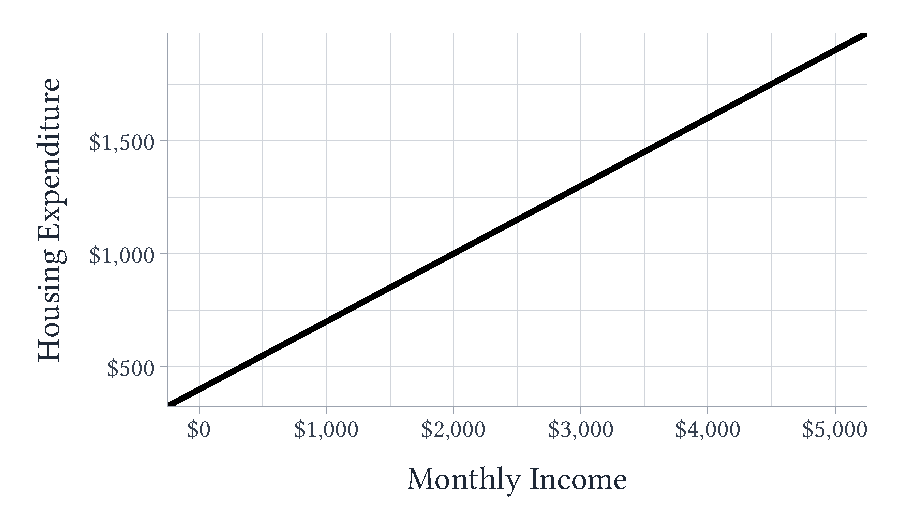
\includegraphics[width = \textwidth]{figures/line_housing.pdf}
      \end{center}
    \end{column}
  \end{columns}
\end{frame}

\begin{frame}{Predictions}
  The first thing we can do is plug in a specific income, say $\kelly{\$2500}$, and determine the housing expenditures:
  $$
    \text{Housing Expenditure} = 400 + 0.35 * \kelly{2500} = \$1275
  $$

  \begin{itemize}
    \item When our line is a \emph{fitted model}, we call these predictions \emph{fitted values} as you take the value of your explanatory variables and use the model fit to predict the value of the outcome variable
  \end{itemize}
\end{frame}

\begin{frame}{Marginal Effects}
  Also, we can think about changing someone's income and seeing how the outcome variable changes. Say you change from $x_1$ to $x_2$, how does $y$ change in response?
  \begin{align*}
    y_2 - y_1 
    &= (\beta_0 + \beta_1 * x_2) - (\beta_0 + \beta_1 * x_1) \\
    &= \beta_1 (x_2 - x_1).
  \end{align*}

  \pause
  \bigskip
  More succinctly, we can write $\Delta y = \beta_1 * \Delta x$
  \begin{itemize}
    \item $\Delta$ (greek for $D$ for ``difference'') takes the difference between the new and old values of the variable
  \end{itemize}
\end{frame}

\begin{frame}{Marginal Effects}
  \vspace*{-2\bigskipamount}
  $$
    y_2 - y_1  = \beta_1 (x_2 - x_1).
  $$

  Notice the slope plays an important role here. It tells us when you change $x$ by a certain amount, then $y$ changes by that amount \emph{scaled} by $\beta_1$. 
  \begin{itemize}
    \item So, if I increase $x$ by one unit, then $y$ changes by $\beta_1$ units
  \end{itemize}

  \pause
  \bigskip
  In our housing example, $\text{Housing Expenditure} = 400 + 0.35 * \text{Monthly Income}$. 
  \begin{itemize}
    \item If I increase my income by $500$, then I change my housing expenditure by $0.35 * 500 = 175$ dollars.
  \end{itemize}
\end{frame}


\subsection*{Multiple variables}

\begin{frame}{Multiple Variables}
  Say we have the following $y = \beta_0 + \beta_1 x_1 + \beta_2 + x_2$, where $x_1$ and $x_2$ are two explanatory variables. Using simlar math above, show that 
  $$
    \Delta y = \beta_1 \Delta x_1 + \beta_2 \Delta x_2
  $$
\end{frame}

\begin{frame}{Marginal Effects}
  \vspace*{-2\bigskipamount}
  $$
    \Delta y = \beta_1 \Delta x_1 + \beta_2 \Delta x_2
  $$

  How does $y$ change when you change $x_1$ while holding $x_2$ equal?
  \begin{itemize}
    \item We have $\Delta x_2 = 0$, so $\Delta y = \beta_1 \Delta x_1$ just like before. 

    \item Called `marginal effect' because we only change one variable, holding the rest fixed.
  \end{itemize}
\end{frame}

\begin{frame}{Example: Predicting Quantity Demanded}
  Consider the example of quantity demanded $Q$ being a linear function of product price $p$ and disposable income $I$:
  $$
    Q = 120 - 9.8 * p + 0.03 * I
  $$

  Say disposable income stays fixed at $\$900$ but the price increases from 8 to 9 dollars. How will the quantity demanded change?
  \pause
  \begin{align*}
    \Delta Q 
    &= -9.8 * \Delta p + 0.03 * \Delta I \\
    &= -9.8 * 1 + 0.03 * 0 = -9.8 \text{ units}
  \end{align*}
\end{frame}


\subsection*{Quadratic Functions}

\begin{frame}{Quadratic model}
  Now say you model the relationship between $x$ and $y$ with a quadratic function
  $$
    y = \beta_0 + \beta_1 x + \beta_2 x^2
  $$

  \bigskip
  Adding polynomial terms allows the relationship between $x$ and $y$ to not be linear 
\end{frame}

\begin{frame}{Example of Quadratic Function}
  \begin{columns}[T]
    \begin{column}{.60\textwidth}\vspace*{-\bigskipamount}
      \begin{center}
    		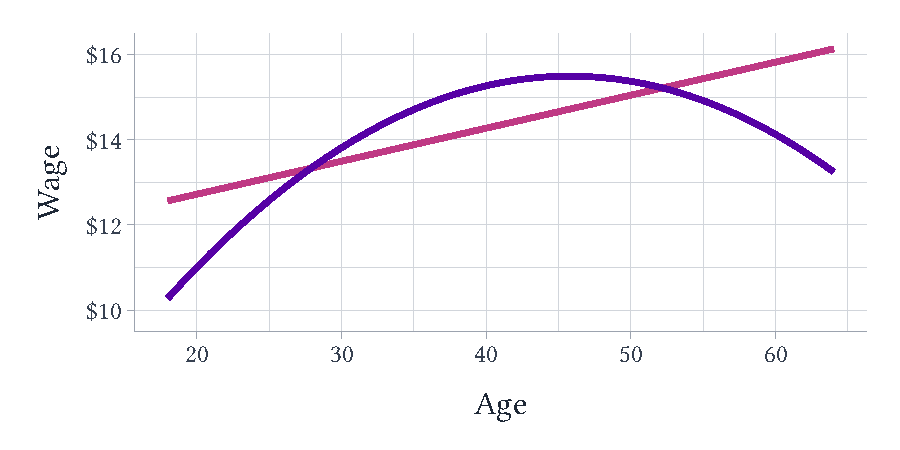
\includegraphics[width=\textwidth]{figures/wage_models.pdf}
      \end{center}
    \end{column}
    \begin{column}{.40\textwidth}
      The quadratic equation better represents the facts that (i) workers are promoted more often at younger ages (quicker wage growth) and (ii) earnings peek around age 45 for workers.
    \end{column}
  \end{columns}
\end{frame}

\begin{frame}{Marginal Effects}
	The equation for wages is given by 
	$$
		\text{Wage} = -5.5 + 1 * \text{Age} - 0.01 * \text{Age}^2
	$$

	Given this equation, how do wages change as a person ages? 
	
	\pause
	Using similar math from before, we can show:
	$$
		\Delta \text{Wage} = \left( 1 - 2 * 0.01 * \text{Age} \right) \Delta \text{Age}
	$$
\end{frame}

\begin{frame}{Marginal Effects}
	\vspace*{-2\bigskipamount}
	$$
		\Delta \text{Wage} = \left( 1 - 2 * 0.01 * \text{Age} \right) \Delta \text{Age}
	$$

	\bigskip
	How much wages change depend on what the worker's current age is
	\begin{itemize}
		\item Moving from 25 to 30, wages increase by $(1 - 2 * 0.01 * 25) * (30 - 25) = +\$2.50$
	
		\pause
		\item Moving from 55 to 60, wages decrease by $(1 - 2 * 0.01 * 55) * (60 - 55) = -\$0.50$.
	\end{itemize}
\end{frame}


\begin{frame}{Marginal Effects}
	More generally, the formula is given by 
	$$
	\Delta y = \underbrace{(\beta_1 + 2 * \beta_2 * x)}_{\text{depends on starting } x} * \Delta x 
	$$
\end{frame}


\subsection*{\texorpdfstring{$\log$}{log} transformations}

\begin{frame}{$\log$ transformation}
	Sometimes it is beneficial to log either the outcome and/or explanatory variables. $\log$-transformations change how we interpret the regression line, namely by changing from `unit' changes to `percent' changes.
	
	\pause
	\bigskip
	E.g. I could model $\log(\text{Wages})$ as a linear regression of age
	\begin{itemize}
		\item My interpretation would be that increasing age by 1 year would increase wages by $\beta_1 * 100$ percent.
	\end{itemize}
\end{frame}

\begin{frame}{Summary of log-transformed linear equations}
	There are four models to consider

	\bigskip
	\begin{tabular}{@{}
		p{0.3\textwidth} p{0.6\textwidth}
	@{}}
		\toprule
		\textbf{Model} & \textbf{Interpretation} \\

		\addlinespace[1mm]
		\midrule
		\addlinespace[1mm]

		$y = \beta_0 + \beta_1 x$ & 
		{\small A 1 unit increase in $x$ increases $y$ by $\beta_1$ units} \\

		$\log(y) = \beta_0 + \beta_1 x$ & 
		{\small A 1 unit increase in $x$ increases $y$ by $\beta_1 * 100$ percent} \\

		$y = \beta_0 + \beta_1 \log(x)$ & 
		{\small A 1 percent increase in $x$ increases $y$ by $\beta_1$ units} \\

		$\log(y) = \beta_0 + \beta_1 \log(x)$ & 
		{\small A 1 percent increase in $x$ increases $y$ by $\beta_1 * 100$ percent} \\

		\bottomrule
	\end{tabular}

	\bigskip
	We derive this in the review notes.
\end{frame}






\section{Review of Statistics and Probability}
\subsection*{Single Random Variables}



\begin{frame}{Key Concepts in Probability}
  Two key concepts in probability:
  \begin{itemize}
    \item \alert{Experiment}: The source of randomness in the world (e.g. flip a coin, roll a dice, play a basketball game)
    \item \alert{Random Variable}: Assigns numerical values determined by an experiment (e.g. value of a die roll, outcome of a game)
  \end{itemize}
\end{frame}

\begin{frame}{Notation for Random Variables}
  Notation for random variables:
  \begin{itemize}
    \item Upper case letters ($W$, $X$, $Y$, $Z$) denote random variables
    \item Lower case letters ($w$, $x$, $y$, $z$) denote particular values \emph{realized} by the random variables
  \end{itemize}
\end{frame}

\begin{frame}{Random Variables in Coin Flipping}
  Example: Coin Flipping Experiment

  \bigskip
  $X$ denotes the random variable counting the number of heads in 10 flips
  \begin{itemize}
    \item $X$ represents the \emph{process of running the experiment}, \emph{not a particular value}
    \item $X$ can take on values in the set ${0, 1, 2, \dots, 10}$
    \item For a particular trial, $X$ takes on a specific value, e.g. $x = 6$
  \end{itemize}
\end{frame}

\subsection*{Discrete Random Variables}

\subsubsection*{Distribution}

\begin{frame}{Discrete random variables}
  A random variable is a \alert{discrete random variable} when it takes on a finite amount of \emph{distinct} values. E.g.:
  \begin{itemize}
    \item Number of heads out of 10 coin flips
    
    \item Student's final letter grade

    \item Whether a candidate wins an election (= 1) or not (= 0)
  \end{itemize}
\end{frame}

\begin{frame}{Probability Density Function}
  The \alert{probability density function} (PDF) assigns probabilities for $X$ obtaining any particular value:
  
  \bigskip 
  Formally, for each possible value $x_j$ of $X$, the PDF is defined as:
  $$
    f_{X}(x_j) = \P{X = x_j} = p_j
  $$
\end{frame}

\begin{frame}{Example pdf}
  Say you flip a single coin and assign $X$ to equal 1 if the coin lands on heads and 0 if it lands on tails. 
  \bigskip
  The pdf for this random variable is $f(1) = 1/2$ and $f(0) = 1/2$.
\end{frame}

\begin{frame}{Example pdf}
  Say you flip a single coin 3 times and record the number of heads in a random variable $Y$. The PDF is given by:
  \begin{align*}
    P_Y(0) &= 1/8 \\
    P_Y(1) &= 3/8 \\
    P_Y(2) &= 3/8 \\
    P_Y(3) &= 1/8 \\
  \end{align*}
\end{frame}

\begin{frame}{Properties of the Probability Density Function (PDF)}
  Two Rules for the PDF:
  \begin{enumerate}
    \item $0 \leq f_{X}(x_j) \leq 1$ for all values of $x_j$ (probability of each value is between 0 and 1)
  
    \pause
    \item $\sum_{j} f_{X}(x_j) = 1$ (sum of probabilities over all possible values equals 1)
  \end{enumerate}
\end{frame}

\begin{frame}{Cumulative Distribution Function (CDF)}
  The cumulative distribution function (CDF) is similar to the PDF but asks about the probability that $X$ takes a value less than or equal to some $x$:
  \[
    F_{X}(x) = \P(X \leq x)
  \]
\end{frame}

\begin{frame}{Example CDF}
  Take a random variable, $Y$ with pdf of $p_1 = \P{Y = 1} = 0.2$, $p_2 = \P{Y = 2} = 0.5$, and $p_3 = \P{Y = 4} = 0.3$. 
  What is the CDF? \pause
  $$
    F_{y}(y) = \begin{cases}
      0.0   \quad \text{when } y < 1, \\
      0.2 \quad \text{when } 1 \leq y < 2, \\
      0.7 \quad \text{when } 2 \leq y < 4, \\
      1.0   \quad \text{when } y \geq 4, \\
    \end{cases}
  $$
\end{frame}

\begin{frame}{Properties of the Cumulative Density Function (CDF)}
  Two Rules for the CDF:
  \begin{enumerate}
    \item $0 \leq F_{X}(x) \leq 1$
    
    \pause
    \item $F_{X}(x)$ is (weakly) increasing in $x$
    \begin{itemize}
      \item $P(X \leq x)$ can not be larger than $P(X \leq x + \text{ a little})$
    \end{itemize}
  \end{enumerate}
\end{frame}

\begin{frame}{Probability Density Function and Statistics}
  The probability density function (pdf) provides a complete picture about a random variable, but it can often be too much information.
  \begin{itemize}
    \item Plotting the pdf as a histogram can still be overwhelming.
  \end{itemize}
  
  \pause
  \bigskip
  To summarize a random variable, we use \alert{statistics} of the data
\end{frame}

\subsubsection*{Expectation}

\begin{frame}{Expectation (Mean)}
  The most common statistic we use is the mean, also known as the \alert{expectation}.
  \begin{itemize}
    \item It answers the question: `what is the average value of some random variable $X$?'
  \end{itemize}
  
  \bigskip 
  The expectation takes the average of the values that $X$ can take, weighted by their probabilities:
  \[
    \expec{X} \equiv \sum_{j=1}^n x_j \P(X = x_j) = \sum_{j=1} x_j p_j
  \]
\end{frame}

\begin{frame}{Example of Expectation}
  Consider a random variable $Y$ with the following pdf:
  \begin{itemize}
    \item $\P(Y = 1) = 0.2$
    \item $\P(Y = 2) = 0.5$
    \item $\P(Y = 4) = 0.3$
  \end{itemize}
  
  \bigskip
  The expectation of $Y$ is:
  \[
    \expec{Y} = 1 \cdot 0.2 + 2 \cdot 0.5 + 4 \cdot 0.3 = 2.4
  \]
\end{frame}

\begin{frame}{Properties of Expectations}
  The following properties of expectations can be derived from the definition of sums:
  \begin{enumerate}
    \item For any constant $c$, $\expec{c} = c$ (no randomness)
    \item For any constant $a$, $\expec{aX} = a \expec{X}$
    \item For any constants $a$ and $b$, $\expec{aX + bY} = a \expec{X} + b \expec{Y}$
  \end{enumerate}
\end{frame}

\begin{frame}{Transformations of Random Variables}
  Consider a function $g$ that transforms a random variable $X$ into a new random variable $Y$, such that $Y = g(X)$
  
  \bigskip 
  The average value of $Y$ can be calculated using the pdf of $X$:
  \[
    \expec{Y} = \expec{g(X)} = \sum_{j=1}^n p_j g(x_j)
  \]
\end{frame}

\subsubsection*{Variance}

\begin{frame}{Variance}
  The other most common statistic is the \alert{variance} of a random variable.

  \bigskip
  While the expectation tells you about the `average' value, the variance tells you about the variability of the random variable:
  \begin{itemize}
    \item The variance measures how much the random variable $X$ moves around its mean
    \item A large variance means the variable moves around a lot
  \end{itemize}
\end{frame}

\begin{frame}{Variance Formula}
  The variance of a random variable $X$ is given by:
  \[
    \var{X} \equiv \expec{\left( X - \expec{X} \right)^2 } = \sum_j p_j (x_j - \expec{X})^2,
  \]
  where the last equality comes from the $g(X)$ rule
\end{frame}

\begin{frame}{Intuition behind Variance}
  \vspace*{-2\bigskipamount}
  \[
    \var{X} \equiv \expec{\left( X - \expec{X} \right)^2 } = \sum_j p_j (x_j - \expec{X})^2,
  \]

  \bigskip
  The intuition behind the variance is as follows:
  \begin{itemize}
    \item $x_j - \expec{X}$ measures how far a particular $x$ value is from the expected value
    
    \pause
    \item If we just used the difference, positives and negatives would cancel out, making it a bad measure of variability
    
    \item Therefore, we square the term to make it positive everywhere, which gives us a good measure of variability
  \end{itemize}
\end{frame}

\begin{frame}{Standard Deviation}
  The \alert{standard deviation} is the square-root of the variance:
  \[
    \sd{X} \equiv \sqrt{\var{X}}
  \]
\end{frame}
  
\begin{frame}{ Properties of Variance}
  In your own time, verify the following properties of variance:
  \begin{enumerate}
    \item For any constant $c$, $\var{c} = 0$
    \item For any constants $a$ and $b$, $\var{aX + b} = a^2 \var{X}$
  \end{enumerate}
\end{frame}

\subsubsection*{Normal Distribution}
\begin{frame}{Normal Distribution}
  The normal distribution is one of the most important distributions in statistics. When a variable is normally distributed, we write $X \sim \mathcal{N}(\mu, \sigma^2)$, where $\mu = \expec{X}$ and $\sigma^2 = \var{X}$.
  \begin{itemize}
    \item The normal distribution is symmetric and the density function of the normal distribution looks like a `bell'
  
    \item The parameter $\mu$ changes where the center of the distribution is and $\sigma^2$ determines how wide the distribution is
  \end{itemize}
\end{frame}

\begin{frame}{Example pdf of different normal distributions}
  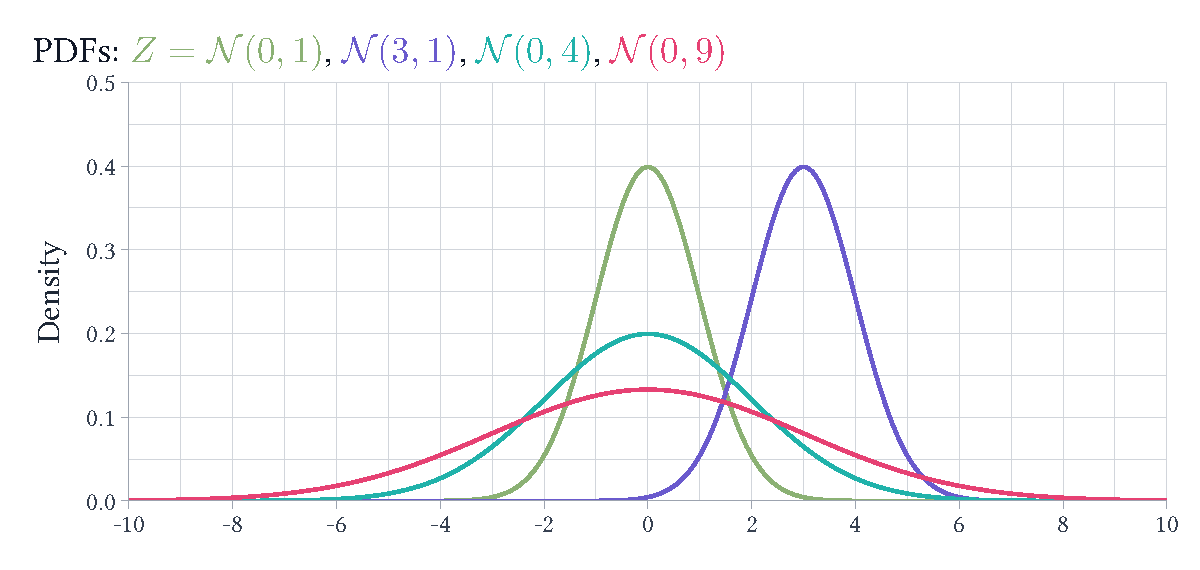
\includegraphics[width = \textwidth]{figures/ex_normal_dist.pdf}
\end{frame}

\begin{frame}{Normal Distribution PDF}
  We can calculate probabilities of taking values $X \in [\ubar{x}, \bar{x}]$ by integrating the area under the PDF. The PDF is given by
  \pause
  $$
    f_X(x) = \frac{1}{\sigma\sqrt{2\pi}} \exp\left( -\frac{1}{2}\left(\frac{x-\mu}{\sigma}\right)^{\!2}\,\right).
  $$
  \bigskip
  Would you want to integrate this function? My guess is probably not.
\end{frame}

\begin{frame}{Z-table and Standard Normal Distribution}
  Instead, we refer to the $Z$-table which calculates probabilities for the \textbf{standard normal distribution} denoted $Z = \mathcal{N}(0, 1)$.
  
  \
  The $Z$-table calculates $P(Z \leq z)$ for values of $z$ ranging from $-3$ to $3$.

  \bigskip
  \pause
  Since we do not have a \emph{standard} normal distribution, we can \textbf{standardize} our variable $X$ to make it standard normal:
  $$
    \frac{X - \mu}{\sigma} \sim Z = \mathcal{N}(0, 1)
  $$
\end{frame}

\begin{frame}{Example: Standardizing and Using Z-table}
  Say we have $X \sim \mathcal{N}(10, 4)$ and we want to know $\prob{X \leq 12}$. Then we can standardize our problem:
  $$
    \prob{X \leq 12} = \prob{\frac{X - 10}{2} \leq \frac{12 - 10}{2}} = \prob{Z \leq 1} 
  $$
  
  \pause
  \bigskip
  The last probability we can find in our $Z$-table by looking up the z-score of $1$. 
\end{frame}

\begin{frame}
  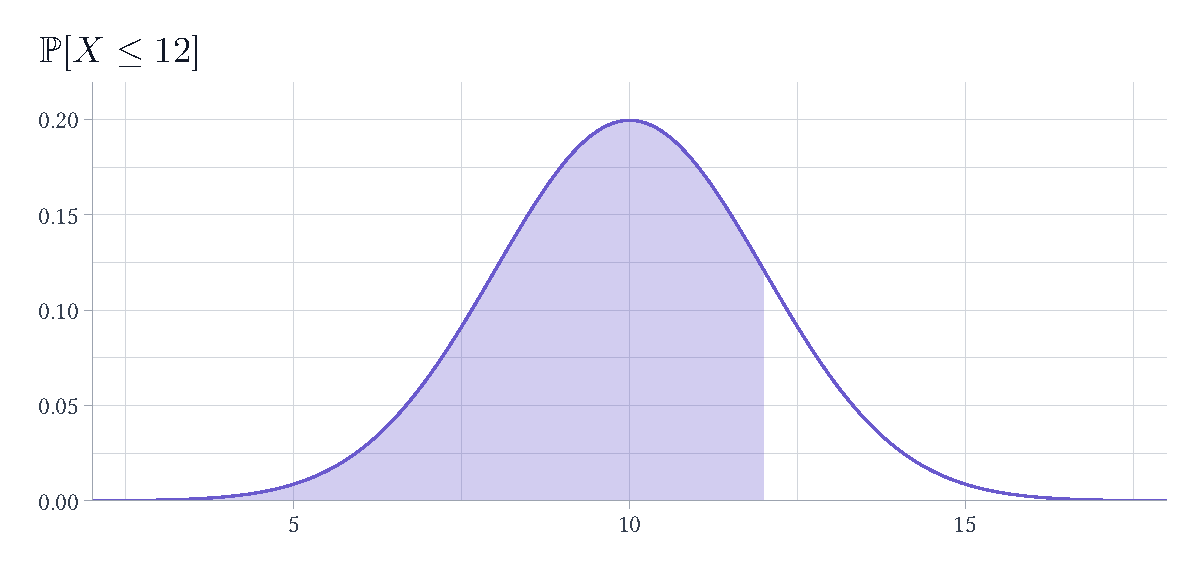
\includegraphics[width = \textwidth]{figures/ex_probability_leq.pdf}
\end{frame}

\begin{frame}
  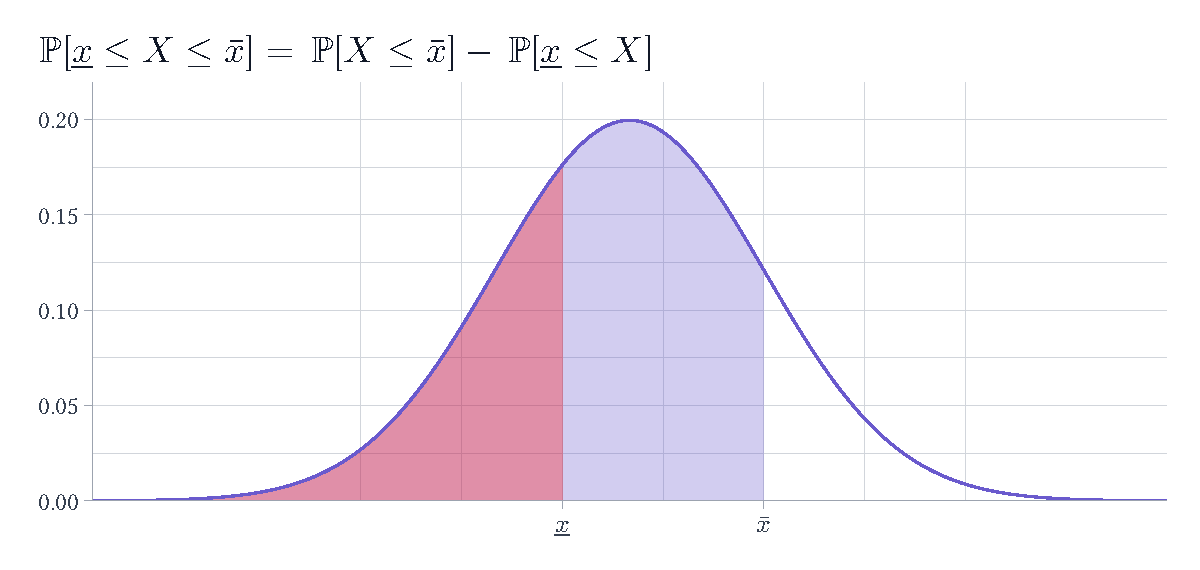
\includegraphics[width = \textwidth]{figures/ex_probability_between.pdf}

  Arbitrary intervals like $[\ubar{x}, \bar{x}]$ can be calculated as $\prob{X \leq \bar{x}} - \prob{X \leq \ubar{x}}$.
\end{frame}



\subsection*{Continuous Random Variables}
\subsubsection*{Distribution}

\begin{frame}{Continuous Random Variables}
  Now we turn to \alert{continuous random variables}, where random variables can take values on (parts of) the real number line (e.g. height).
  \begin{itemize}
    \item All our definitions and intuition still apply.

    \item In continuous land, we move from sums $\sum$ to integrals $\int$.
  \end{itemize}
\end{frame}

\begin{frame}{Probability Density Function}
  For continuous random variables, The PDF no longer represents the probability that $X$ obtains the value $x$, since the probability of obtaining any particular value is 0
  \begin{itemize}
    \item Instead, the pdf gives a `relative likelihood' that you take a value ``near $x$''
  \end{itemize}

  \pause
  \bigskip
  The pdf can be used to find the probability of being in a range of values $[\ubar{x}, \bar{x}]$:
  \[
    \P{X \leq x} = \int_{\ubar{x}}^{\bar{x}} f_{X}(x) dx,
  \]
\end{frame}

\begin{frame}{Cumulative Distribution Function}
  The PDF can be used to find the cumulative distribution function (CDF):
  \[
    \P{X \leq x} = \int_{-\infty}^x f_{X}(x) dx,
  \]
\end{frame}


\begin{frame}{Expectations for Continuous Random Variables}
  For continuous random variables, the expectation takes the form:
  \[
    \E{X} = \int x * f_{X}(x) dx.
  \]
  \begin{itemize}
    \item This is similar to the discrete case, but we use an integral to `average' the value times the density
  \end{itemize}

  \pause
  \bigskip
  All the properties of expectations listed above hold for continuous variables too (or mixtures of both).
\end{frame}

\begin{frame}{Variance for Continuous Random Variables}
  Last, the variance is given by
  $$
    \var{X} = \int (x - \expec{X})^2 f_{X}(x) dx
  $$
\end{frame}

\section{Multiple Random Variables}

\begin{frame}{Joint Distributions}
  In this class, we care about how variables \emph{relate to one another}. For example:
  \begin{itemize}
    \item Do sales grow and shrink with a consumer's age?
    
    \item Is height an important predictor of basketball success?
    
    \item Is the sale associated with a large increase in sales?
  \end{itemize}

  \pause
  \bigskip
  To answer these questions, we need to know about the \alert{joint distribution} between two variables $X$ and $Y$.
\end{frame}

\begin{frame}{Joint Probability Density Function}
  The \alert{joint probability density function} is denoted by $f_{X,Y}(x, y)$:
  
  \bigskip
  In the discrete case, it is the probability that $X = x$ \emph{and} $Y = y$ \emph{in the same trial}:
  \[
    f_{X,Y}(x, y) = \P{X = x, Y = y}.
  \]
\end{frame}

\begin{frame}{Conditional Probability Density Function}
  We can also think about \alert{conditioning} on the value of one of the random variables

  \bigskip
  Take $Y$ to be \emph{fixed} to some value $y$. Then we could ask about the distribution of $X$ \emph{within trials where $Y = y$}:
  \[
    f_{X \vert Y}(x \vert y) = \P{X = x}{Y = y}
  \]

  \pause
  \begin{itemize}
    \item Note we use the $\vert$ symbol to note `conditioning' on some random variable's realization
    
    \pause
    \item In our example, we learn that $Y = y$ for that trial and then ask about the (conditional) probability that $X = x$
  \end{itemize}
\end{frame}

\begin{frame}{Bayes Rule}
  The \alert{Bayes Rule} helps us translate between conditional pdfs and joint pdfs:
  \[
    f_{X \vert Y}(x \vert y) = f_{X,Y}(x, y) / f_{Y}(y).
  \]
  
  \pause
  \bigskip
  So say we have two discrete random variables and we want to know the probability $X = x$ conditional on $Y = y$. We can calculate it if we know:
  \begin{enumerate}
    \item the probability that $Y = y$
    \item the joint probability that $Y = y$ \emph{and} $X = x$
  \end{enumerate}
\end{frame}

\subsection*{Covariance and Correlation}

\begin{frame}{Covariance and Correlation}
  Similar to how we used statistics to summarize a single random variable, it is common to want to summarize how two variables are related to one another.
  \begin{itemize}
    \item For this, we use the \alert{covariance} or the \alert{correlation} between two variables (they are very similar)
  \end{itemize}
\end{frame}

\begin{frame}{Covariance}
  The covariance looks like the variance of a random variable:
  \[
    \cov(X, Y) = \mathbb{E}\left[ (X - \expec{X}) (Y - \expec{Y}) \right]
  \]
  The covariance intuitively measures whether $X$ and $Y$ move together:
  \begin{itemize}
    \item The covariance is positive if when $X$ is above its mean, $Y$ also tends to be above its mean; and when $X$ is below its mean, $Y$ also tends to be below its mean
    \item They ``co-move'' together
  \end{itemize}
\end{frame}

\begin{frame}{Covariance}
  The covariance is negative if when $X$ is above its mean, $Y$ tends to be below its mean and vice versa
  \begin{itemize}
    \item They move in opposite directions, but are still related!
    
    \pause
    \item In other words, if I know $X$ was above its mean, then I would predict that $Y$ is below its mean (knowing one gives me information on the other)
  \end{itemize}
\end{frame}

\begin{frame}{Alternative Formula for Covariance}
  With some algebra and the rules of expectations, we can see:
  \begin{align*}
    \cov(X, Y) 
    &= \mathbb{E}\left[ (X - \expec{X}) (Y - \expec{Y}) \right] \\
    &= \mathbb{E}\left[ XY - \expec{X} Y - X \expec{Y} + \expec{X} \expec{Y} \right] \\ 
    &= \expec{XY} - \expec{X} \expec{Y} - \expec{X} \expec{Y} + \expec{X} \expec{Y} \\
    &= \expec{XY} - \expec{X} \expec{Y}.
  \end{align*}
\end{frame}

\begin{frame}{Correlation}
  The correlation is just a rescaled version of the covariance:
  \[
    \corr(X, Y) = \frac{\cov(X, Y)}{\sd{X} \sd{Y}}.
  \]

  \bigskip
  The correlation is designed to always be between -1 and 1 (because of the rescaling):
  \begin{itemize}
    \item It is more popular since people are used to thinking about correlations.
    \item A correlation close to 1 and/or -1 is a \emph{very strong} relationship.
  \end{itemize}
\end{frame}

\begin{frame}{Limitations of Covariance and Correlation}
  It is important to know that covariance and correlation only measure a \emph{linear} relationship between $X$ and $Y$:
  \begin{itemize}
    \item If the function connecting $X$ and $Y$ is non-linear, then the correlation is a bad summary statistic of the relationship between them.
    
    \item This is similar to how the mean is a bad measure for highly skewed data.
  \end{itemize}
\end{frame}

\subsubsection*{Independence}

\begin{frame}{Independence}
  Two random variables are said to be \alert{independent} if knowing information about the realization of one of them tells you nothing about the realization of the other one.
  
  \pause
  \bigskip
  For example, if I told you the day was Sunday ($X = $ Sunday), then you would not have any better prediction about whether it is raining ($Y = 1$)
  \begin{itemize}
    \item The two random variables are independent
  \end{itemize}
\end{frame}

\begin{frame}{Independence and Conditional Probability}
  When $X$ and $Y$ are independent, this can be summarized by:
  \[
    f_{X \vert Y}(x \vert y) = f_{X}(x).
  \]

  \pause
  \bigskip
  This also implies that when $X$ and $Y$ are independent,
  \[
    F_{X,Y}(x, y) = F_{X}(x) F_{Y}(y).
  \]
\end{frame}

\begin{frame}{Properties of Independent Random Variables}
  Using the definition of expectations, we can derive the following when $X$ and $Y$ are independent:
  \begin{itemize}
    \item $\expec{XY} = \expec{X} \expec{Y}$
    \item $\cov(X, Y) = 0$
    
    \pause
    \item $\var{aX + bY} = a^2 \var{X} + b^2 \var{Y}$
  \end{itemize}
  
  \bigskip
  The last fact comes from the fact that for \emph{all} random variables $\var{aX + bY} = a^2 \var{X} + b^2 \var{Y} + 2ab \cov(X, Y)$, but the last term is zero from independence.
\end{frame}



\section{Statistical Inference}

\begin{frame}{Statistical Inference}
  \alert{Statistical Inference} is the procedure of using a random sample of observations from a population to try and learn some summary of the population distribution of the data.

  \pause
  \bigskip
  To be more specific, there is some \alert{statistic} of the population distribution (e.g. it's expectation, it's variance, the 80th percentile, etc.)
  \begin{itemize}
    \item We will call the target statistic $\theta$
  \end{itemize}
\end{frame}

\subsection*{Estimators}

\begin{frame}{Estimating Population Statistics}
  We do not observe the full population; only \alert{a random sample}, $X_1, \dots, X_n$. We take our data and calculate an \alert{estimate} of the population statistic $\theta$
  \begin{itemize}
    \item The calculation we choose is called our \alert{estimator}.
  \end{itemize}

  \pause
  \bigskip
  For example, we can use the sample average from a set of observations to infer about the expectation of the population. To do so, we chose the sample average as our estimator:
  $$
    \underbrace{\bar{X}}_{\text{Estimator}} \equiv \frac{1}{n} \sum_{i=1}^n X_i
  $$
\end{frame}

\begin{frame}{Sample Distribution of an Estimator: Thought Experiment}
  To understand the \alert{sample distribution} of an estimator, we need a thought experiment called \alert{repeated sampling}. 
  
  \pause
  \bigskip
  In reality, we only have a single sample of size $n$. But, the thought experiment is  is to imagine collecting multiple samples and calculating the estimator for each sample:
  \begin{itemize}
    \item The distribution of estimates across repeated sampling is called the  \textbf{sample distribution}
  \end{itemize}

  \pause
  \bigskip
  The sample distribution can be used to quantify how much our estimator varies across different samples of the same size, $n$
\end{frame}

\begin{frame}{Estimators}
  For any statistic, there are many different estimators. Therefore, we have various ways to discuss what makes a good estimator.
\end{frame}

\begin{frame}{Property 1: Unbiasedness}
  An estimator $W$ is \alert{unbiased} for $\theta$ if:
  $$
    \expec{W} = \theta.
  $$
  \bigskip
  This means that, on average, the estimator equals the population statistic when using repeated sampling.  
  \begin{itemize}
    \item It does not imply that the estimate always equals the population statistic.
  \end{itemize}
  
  \pause
  \bigskip
  For instance, the sample mean is an unbiased estimate of the population mean.
\end{frame}

\begin{frame}{Property 2: Consistency}
  Let $W_n$ be an estimator of $\theta$ based on a sample size $n$. The estimator is \alert{consistent} if, as $n$ increases, $W_n \to \theta$ and the variance of $W_n$ approaches 0.  
  
  \pause
  \begin{itemize}
    \item This means the estimator becomes more precise and centers around the population statistic.
  \end{itemize}
\end{frame}

\begin{frame}{Property 3: Efficiency}
  If $W_1$ and $W_2$ are two unbiased estimators, we say $W_1$ is more efficient than $W_2$ if:
  $$
    \var{W_1} < \var{W_2}
  $$
  
  \bigskip
  This indicates that $W_1$ has a smaller variance, making it a more precise estimator
\end{frame}

\subsection*{Confidence Intervals}

\begin{frame}{Describing Uncertainty of an Estimator}
  Since the estimator does not always equal its population statistic in repeated sampling, we need to describe the uncertainty of an estimator.  
  \begin{itemize}
    \item To do this, we require an estimate of the variability of our estimator in repeated sampling
  \end{itemize}
\end{frame}

\begin{frame}{Normal Distribution and Confidence Intervals}
  It turns out that the \emph{sample distribution} of many estimators is approximately normally distributed
  \begin{itemize}
    \item Makes it easier to summarize uncertainty around the estimator
  \end{itemize}

  \bigskip
  \pause
  A \alert{confidence interval} is constructed to describe the level of certainty
  \begin{itemize}
    \item Centered on the estimate, with a width that describes a range of values the population statistic could be
  \end{itemize}
\end{frame}

\begin{frame}{Sample Mean Distribution}
  Let $\{ Y_1, \dots, Y_n \}$ be a random sample. The sample mean is approximately distributed $\mathcal{N}(\mu, \sigma^2 / n)$ where $\mu = \expec{Y}$ and $\sigma^2 = \var{Y}$. 

  \pause
  We can construct a 95\% confidence interval as: 
  \begin{align*}
    &\P{-1.96 < \frac{\bar{Y} - \mu}{\sigma / \sqrt(n)} < 1.96} = 0.95 \\
    \implies &\P{\bar{Y} - 1.96 * \frac{\sigma}{\sqrt(n)} < \mu  < \bar{Y} + 1.96 \frac{\sigma}{\sqrt(n)}} = 0.95
  \end{align*}
\end{frame}

\begin{frame}{Confidence Interval}
  That is, in repeated sampling, there is a 95\% probability (95 out of 100 samples of size $n$) that $\mu$ falls within our confidence interval: 
  $$
    \left[
      \bar{Y} - 1.96 * \frac{\sigma}{\sqrt(n)}, 
      \bar{Y} + 1.96 \frac{\sigma}{\sqrt(n)}
    \right]
  $$

  \pause
  \bigskip
  Since we do not observe $\sigma$, we will estimate it using the following estimator, called the sample standard deviation of $y$:
  $$
    s = \sqrt{\frac{1}{n-1} \sum_{i=1}^n (Y_i - \bar{Y})^2}
  $$
\end{frame}

\begin{frame}{Critical Values and Confidence Level}
  The values $-1.96$ and $1.96$ are the critical values for the 2.5th percentile and 97.5th percentile of the standard normal distribution, corresponding to a 95\% confidence level.

  \pause
  \bigskip
  To increase the confidence level, we need to use larger critical values. For example, for a 99\% confidence level, we use the 0.5th percentile and 99.5th percentile of the normal distribution for our critical values.
\end{frame}

\begin{frame}{Z-score and Standard Normal Distribution}
  This procedure works because $\bar{Y} \sim \mathcal{N}(\mu, \sigma^2/n)$ and therefore our \textbf{$Z$-score}, $\frac{\bar{Y} - \mu}{\sigma / \sqrt(n)}$, is approximately distributed as the standard normal distribution.
  \begin{itemize}
    \item Therefore using the standard normal distribution to chose critical values works
  \end{itemize}
\end{frame}

\subsection*{Hypothesis Testing}

\begin{frame}{Hypothesis Testing}
  In addition to confidence intervals, it is common to perform \alert{hypothesis tests}. 
  
  \bigskip
  Simply put, we want to test whether evidence is consistent with a \alert{null hypothesis} that $\theta$ equals some value (e.g. we could hypothesize that the population mean height is 5 ft. 8 in.). 
  \begin{itemize}
    \item We then would calculate our sample mean and if it is ``too far'' from the null hypothesis population mean, then we say the evidence rejects the null hypothesis.
  \end{itemize}
\end{frame}

\begin{frame}{Determining "Too Far"}
  How far is ``too far'' away from the null hypothesis? That depends on 
  \begin{enumerate}
    \item how noisy our estimate is (the sample distribution), and 
    
    \item how confident we want to be in rejecting the null
  \end{enumerate}
\end{frame}

\begin{frame}{Test Statistics}
  We will use our sample's estimate to calculate a \alert{test statistic}. The test statistic (a random variable) will be referred to as $T$ and a realized value as $t$. 

  \bigskip
  \emph{When the null hypothesis is true}, the test statistic will be distributed as $\mathcal{N}(0, v)$ (normally distributed with mean $0$ and some variance $v$). 
  \pause
  \begin{itemize}
    \item Therefore, we expect $T$ to be very close to zero (if the null is true)
    
    \item So, if we find a value of $T = t$ that is ``very far'' away from zero, then we find evidence against the null hypothesis
  \end{itemize}
\end{frame}

\begin{frame}{$p$-Value}
  Given a level of confidence (e.g. 95\%) and the variance $v$, we can use properties of the normal distribution to determine the probability that a draw from the $T \sim \mathcal{N}(0, v)$ distribution would be $\geq \abs{\hat{t}}$
  
  \bigskip
  This is called the \textbf{$p$-value}
  \begin{itemize}
    \item In words, the $p$-value tells us, ``assuming the null hypothesis is true, how often would we expect to see a value as large or larger than the one we \emph{did observe in our sample}'' 
  
    \item If that probability is small, then we will reject the null.
  \end{itemize}
\end{frame}

\begin{frame}{Significance Level}
  In particular, given our level of confidence (e.g. 95\%), define the \textbf{significance level} as $\alpha = 1 -$ the level of confidence (e.g. 5\%)
  
  \bigskip
  We reject the null if the $p$-value, $p$ is smaller than the significance level
  \begin{itemize}
    \item Typically, we will use $\alpha = 0.05$
  \end{itemize}
\end{frame}

\begin{frame}{Example: Hypothesis Testing for Sample Mean}
  Let $\{ Y_1, \dots, Y_n \}$ be a random sample. The sample mean is approximately distributed $\mathcal{N}(\mu, \sigma^2 / n)$ where $\mu = \expec{Y}$ and $\sigma^2 = \var{Y}$
  
  \bigskip
  We will test the null hypothesis $H_0: \mu = \mu_0$ for some proposed value $\mu_0$
\end{frame}

\begin{frame}{Example: Hypothesis Testing for Sample Mean}
  Then, our test statistic is given by 
  $$
    T = \frac{\bar{X} - \mu_0}{\hat{\sigma} / \sqrt(n)},
  $$
  where $\hat{\sigma}$ is the square root of our estimate of the variance of $Y$
  \begin{itemize}
    \item Assuming the null hypothesis is true, $H_0$, then $T \sim \mathcal{N}(0, 1)$.
  \end{itemize}
\end{frame}

\begin{frame}{Example: Hypothesis Testing for Sample Mean}
  Therefore, the $p$-value is given by
  $$
    p = \prob{T \geq \abs{t}} = 2 * \prob{Z \leq -\abs{t}},
  $$
  where $Z$ is the standard normal random variable. 
  \pause
  \begin{itemize}
    \item You can find this probability by looking up $-\abs{t}$ in the $Z$-table.
  \end{itemize}
\end{frame}

\begin{frame}{Rejection Region}
  Last, we will discuss the \textbf{rejection region} for a given \emph{null hypothesis}:

  \bigskip
  This is defined as the set of values of our estimate where we would reject the null hypothesis for a given significance level, $\alpha$.
\end{frame}

\begin{frame}{Example: Hypothesis Testing for Sample Mean}
  The rejection region can be found, most simply, by forming a confidence interval around the null hypothesis. Any value \emph{outside this interval} will be rejected.

  \pause
  \bigskip
  Our confidence interval for $\alpha = 0.05$ is given by 
  $$
    \left[ \mu_0 - 1.96 * \sigma/\sqrt{n},  \mu_0 + 1.96 * \sigma/\sqrt{n} \right]
  $$

  \bigskip
  Therefore our rejection region is $\bar{X} \leq \mu_0 - 1.96 * \sigma/\sqrt{n}$ or $\bar{X} \geq \mu_0 + 1.96 * \sigma/\sqrt{n}$.
\end{frame}




\end{document}
